%%%%%%%%%%%%%%%%%%%%%%%%%%%%%%%%%%%%%%%%%
% a0poster Portrait Poster
% LaTeX Template
% Version 1.0 (22/06/13)
%
% The a0poster class was created by:
% Gerlinde Kettl and Matthias Weiser (tex@kettl.de)
% 
% This template has been downloaded from:
% http://www.LaTeXTemplates.com
%
% License:
% CC BY-NC-SA 3.0 (http://creativecommons.org/licenses/by-nc-sa/3.0/)
%
%%%%%%%%%%%%%%%%%%%%%%%%%%%%%%%%%%%%%%%%%

%----------------------------------------------------------------------------------------
%	PACKAGES AND OTHER DOCUMENT CONFIGURATIONS
%----------------------------------------------------------------------------------------

\documentclass[a0,portrait]{a0poster}

\usepackage{multicol} % This is so we can have multiple columns of text side-by-side
\columnsep=100pt % This is the amount of white space between the columns in the poster
%\columnseprule=3pt % This is the thickness of the black line between the columns in the poster

\usepackage[svgnames]{xcolor} % Specify colors by their 'svgnames', for a full list of all colors available see here: http://www.latextemplates.com/svgnames-colors

\usepackage{times} % Use the times font
%\usepackage{palatino} % Uncomment to use the Palatino font

\usepackage{graphicx} % Required for including images
\graphicspath{{figs/}} % Location of the graphics files
\usepackage{booktabs} % Top and bottom rules for table
\usepackage[font=small,labelfont=bf]{caption} % Required for specifying captions to tables and figures
\usepackage{amsfonts, amsmath, amsthm, amssymb} % For math fonts, symbols and environments
\usepackage{wrapfig} % Allows wrapping text around tables and figures
\usepackage{subcaption}
\newcommand{\gpmem}{\texttt{gpmem}}
\newcommand{\emu}{{\textrm{emu}}}
\begin{document}

%----------------------------------------------------------------------------------------
%	POSTER HEADER 
%----------------------------------------------------------------------------------------

% The header is divided into two boxes:
% The first is 75% wide and houses the title, subtitle, names, university/organization and contact information
% The second is 25% wide and houses a logo for your university/organization or a photo of you
% The widths of these boxes can be easily edited to accommodate your content as you see fit
\begin{flushright}
\begin{minipage}[b]{0.25\linewidth}

\includegraphics[width=7cm]{mitlogo.png}
\hspace{1cm}

\includegraphics[width=8cm]{royalhollowaylogo.jpg}
\end{minipage} 
\end{flushright}

\vspace{2cm}

\begin{center}
\addtolength{\tabcolsep}{20pt} 
\veryHuge \textbf{Probabilistic Programming with Gaussian Process Memoization} \color{Black}\\[1.5cm] % Title
 \Large   \begin{tabular}{  c  c  c c}
           \textbf{Ulrich Schaechtle}  & \textbf{Ben Zinberg} & \textbf{Vikash K. Mansinghka} & \textbf{Kostas Stathis}\\ 
           Department of Computer Science & Computer Science \& AI Lab & Computer Science \& AI Lab & Department of Computer Science \\
           Royal Holloway, Univ. of London & Massachusetts Institute of Technology & Massachusetts Institute of Technology & Royal Holloway, Univ. of London \\
        \end{tabular}

\addtolength{\tabcolsep}{-2pt} 
\end{center}



\vspace{3cm} % A bit of extra whitespace between the header and poster content

%----------------------------------------------------------------------------------------

\begin{multicols}{2} % This is how many columns your poster will be broken into, a portrait poster is generally split into 2 columns

%----------------------------------------------------------------------------------------
%	ABSTRACT
%----------------------------------------------------------------------------------------

%\color{Navy} % Navy color for the abstract

\begin{abstract}
The poster describes the {\em Gaussian process memoizer}, a probabilistic programming technique that uses Gaussian processes to provides a statistical alternative to memorization. Memoizing a target procedure results in a “self-caching” wrapper that remembers previously computed values. Gaussian process memoization additionally produces a statistical emulator based on a Gaussian process whose predictions automatically improve whenever a new value of the target procedure becomes available. The work also introduces  an efficient implementation, named {\tt gpmem}, that can use kernels given by a broad class of probabilistic programs. The flexibility of {\tt gpmem} is illustrated via three applications: (i) GP regression with hierarchical hyper-parameter learning, (ii) Bayesian structure learning via compositional kernels generated by a probabilistic grammar, and (iii) a bandit formulation of Bayesian optimization with automatic inference and action selection. All applications share a single 50-line Python library and require fewer than 20 lines of probabilistic code each.
\end{abstract}


\color{DarkSlateGray} % DarkSlateGray color for the rest of the content
%\color{SaddleBrown} % SaddleBrown color for the introduction
%----------------------------------------------------------------------------------------
%	GP Memoization
%----------------------------------------------------------------------------------------
\section*{GP Memoization: {\tt gpmem}}

---------------------------------------------------------------------


%----------------------------------------------------------------------------------------
%	Bayesian GP
%----------------------------------------------------------------------------------------
\section*{Bayesian GP}
\begin{center}\vspace{1cm}
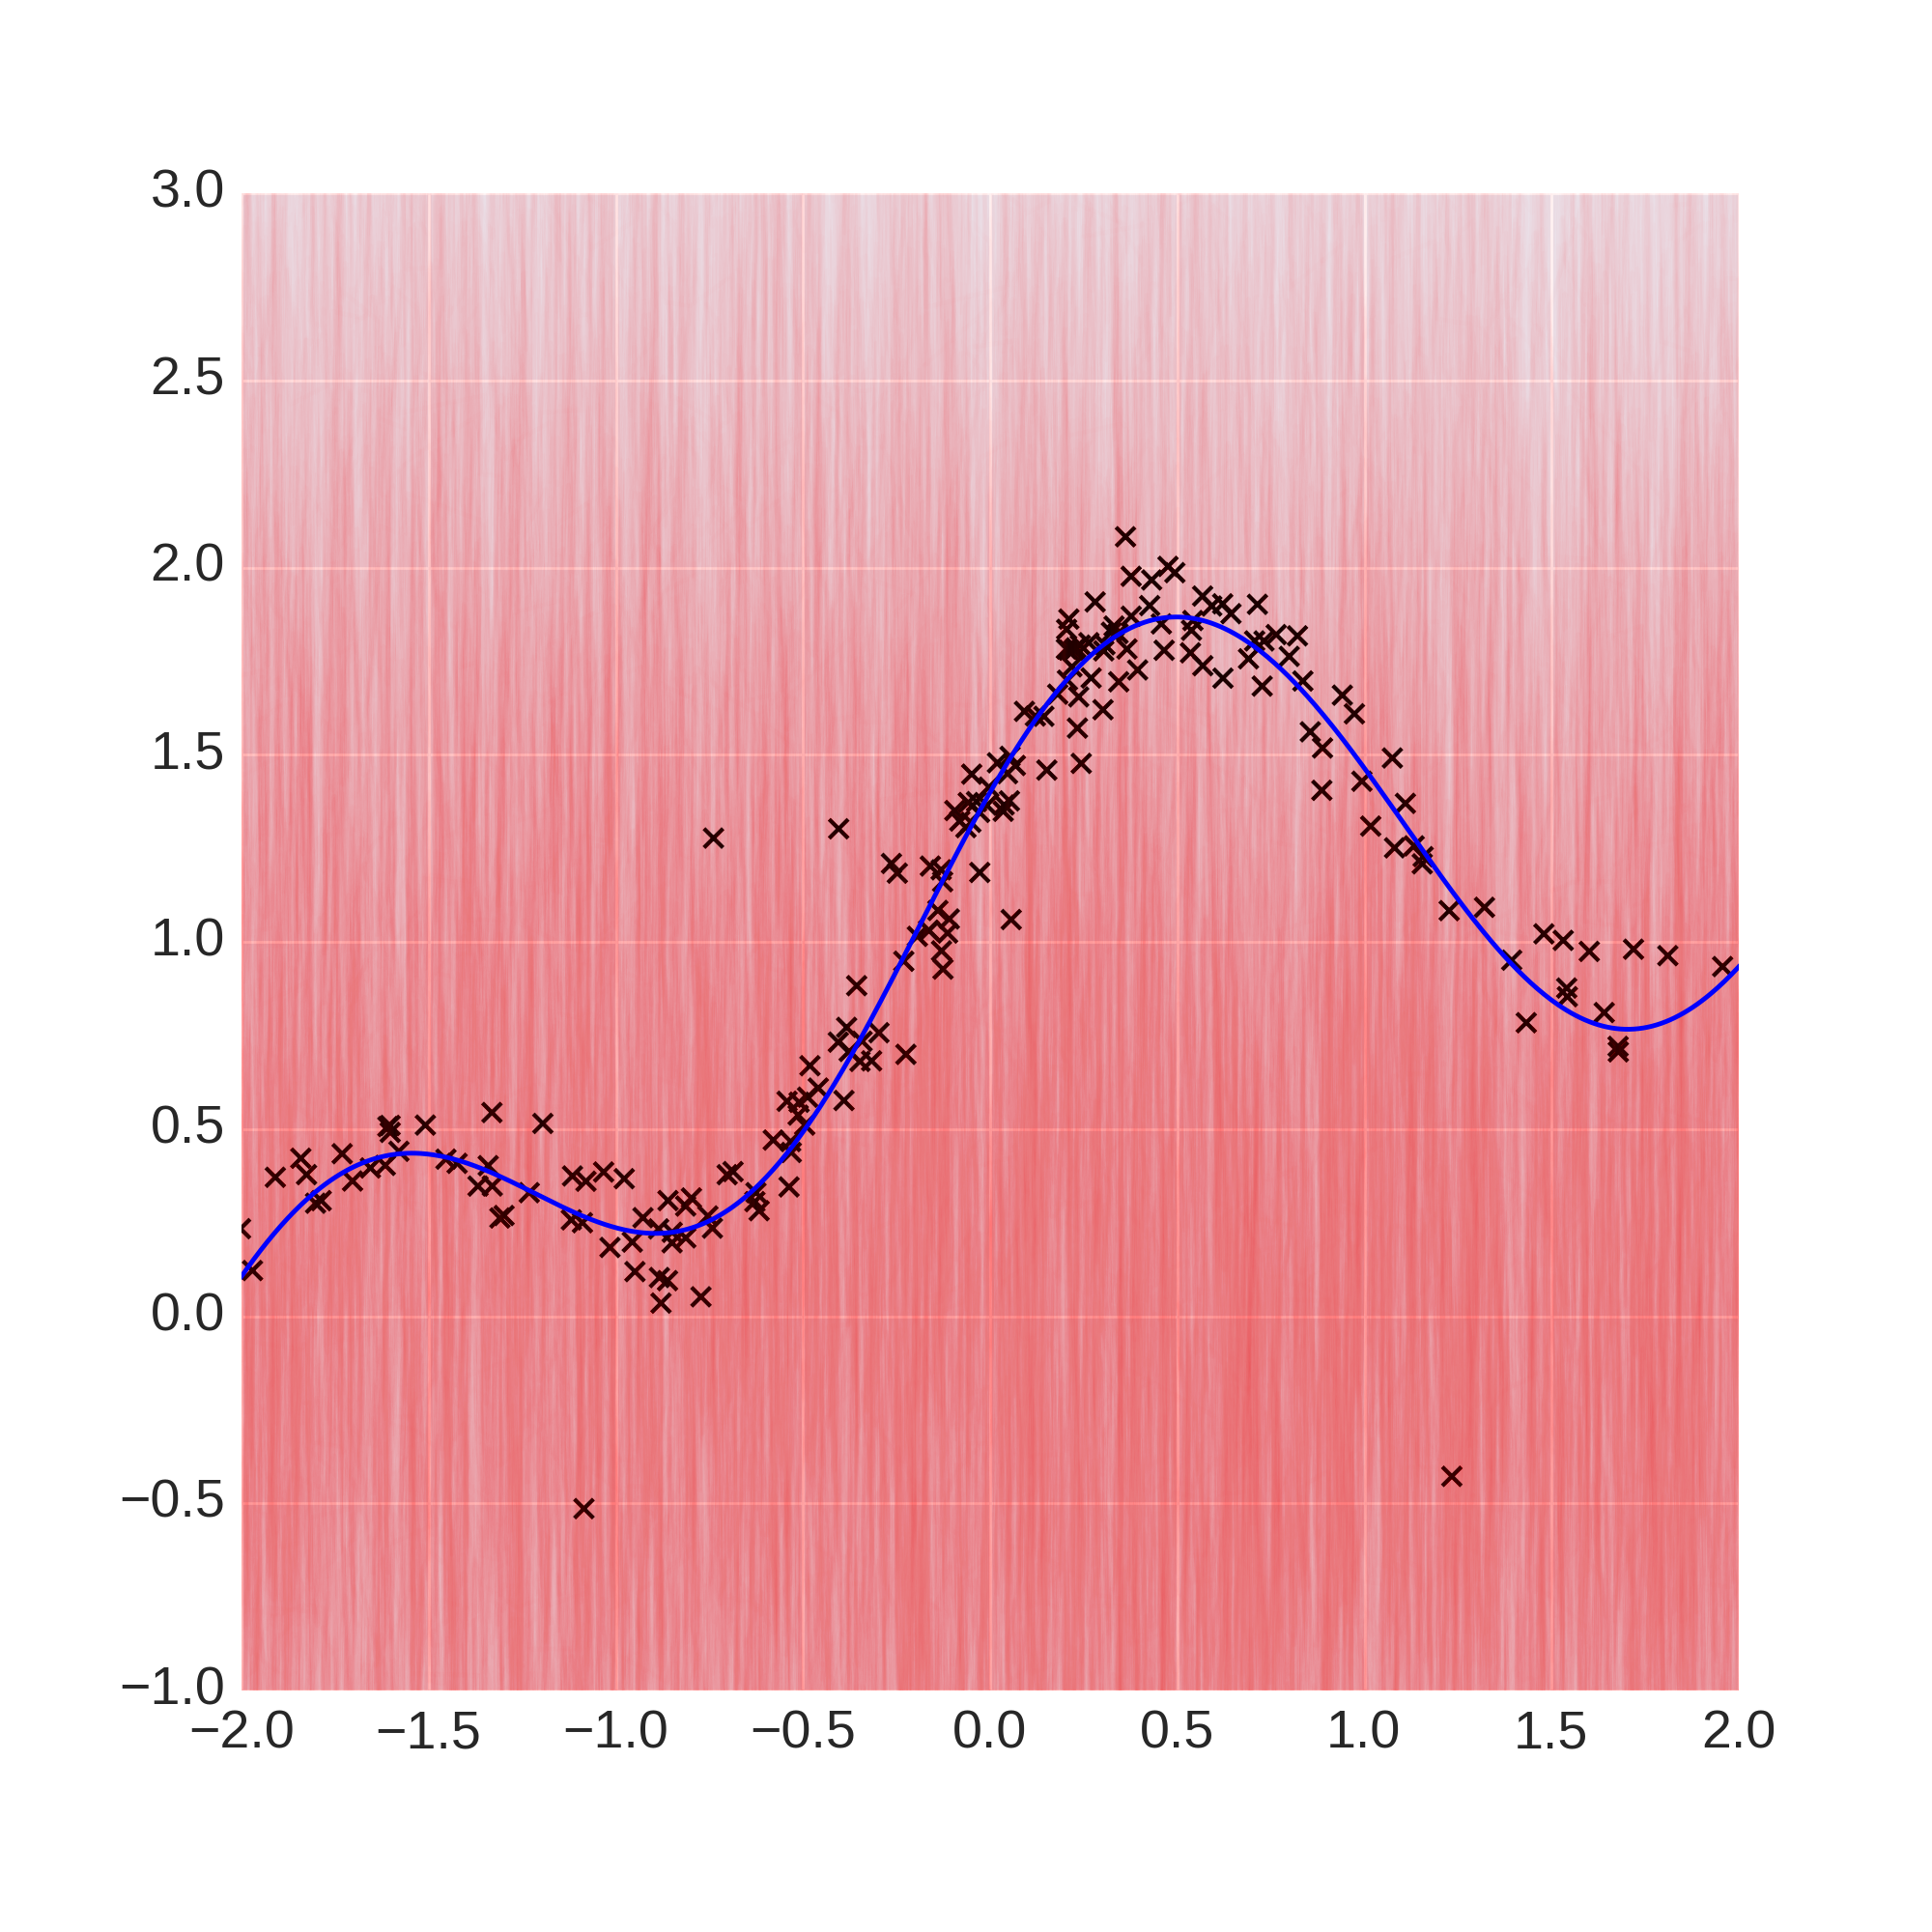
\includegraphics[height=7.5cm]{neal_se_1final.png}
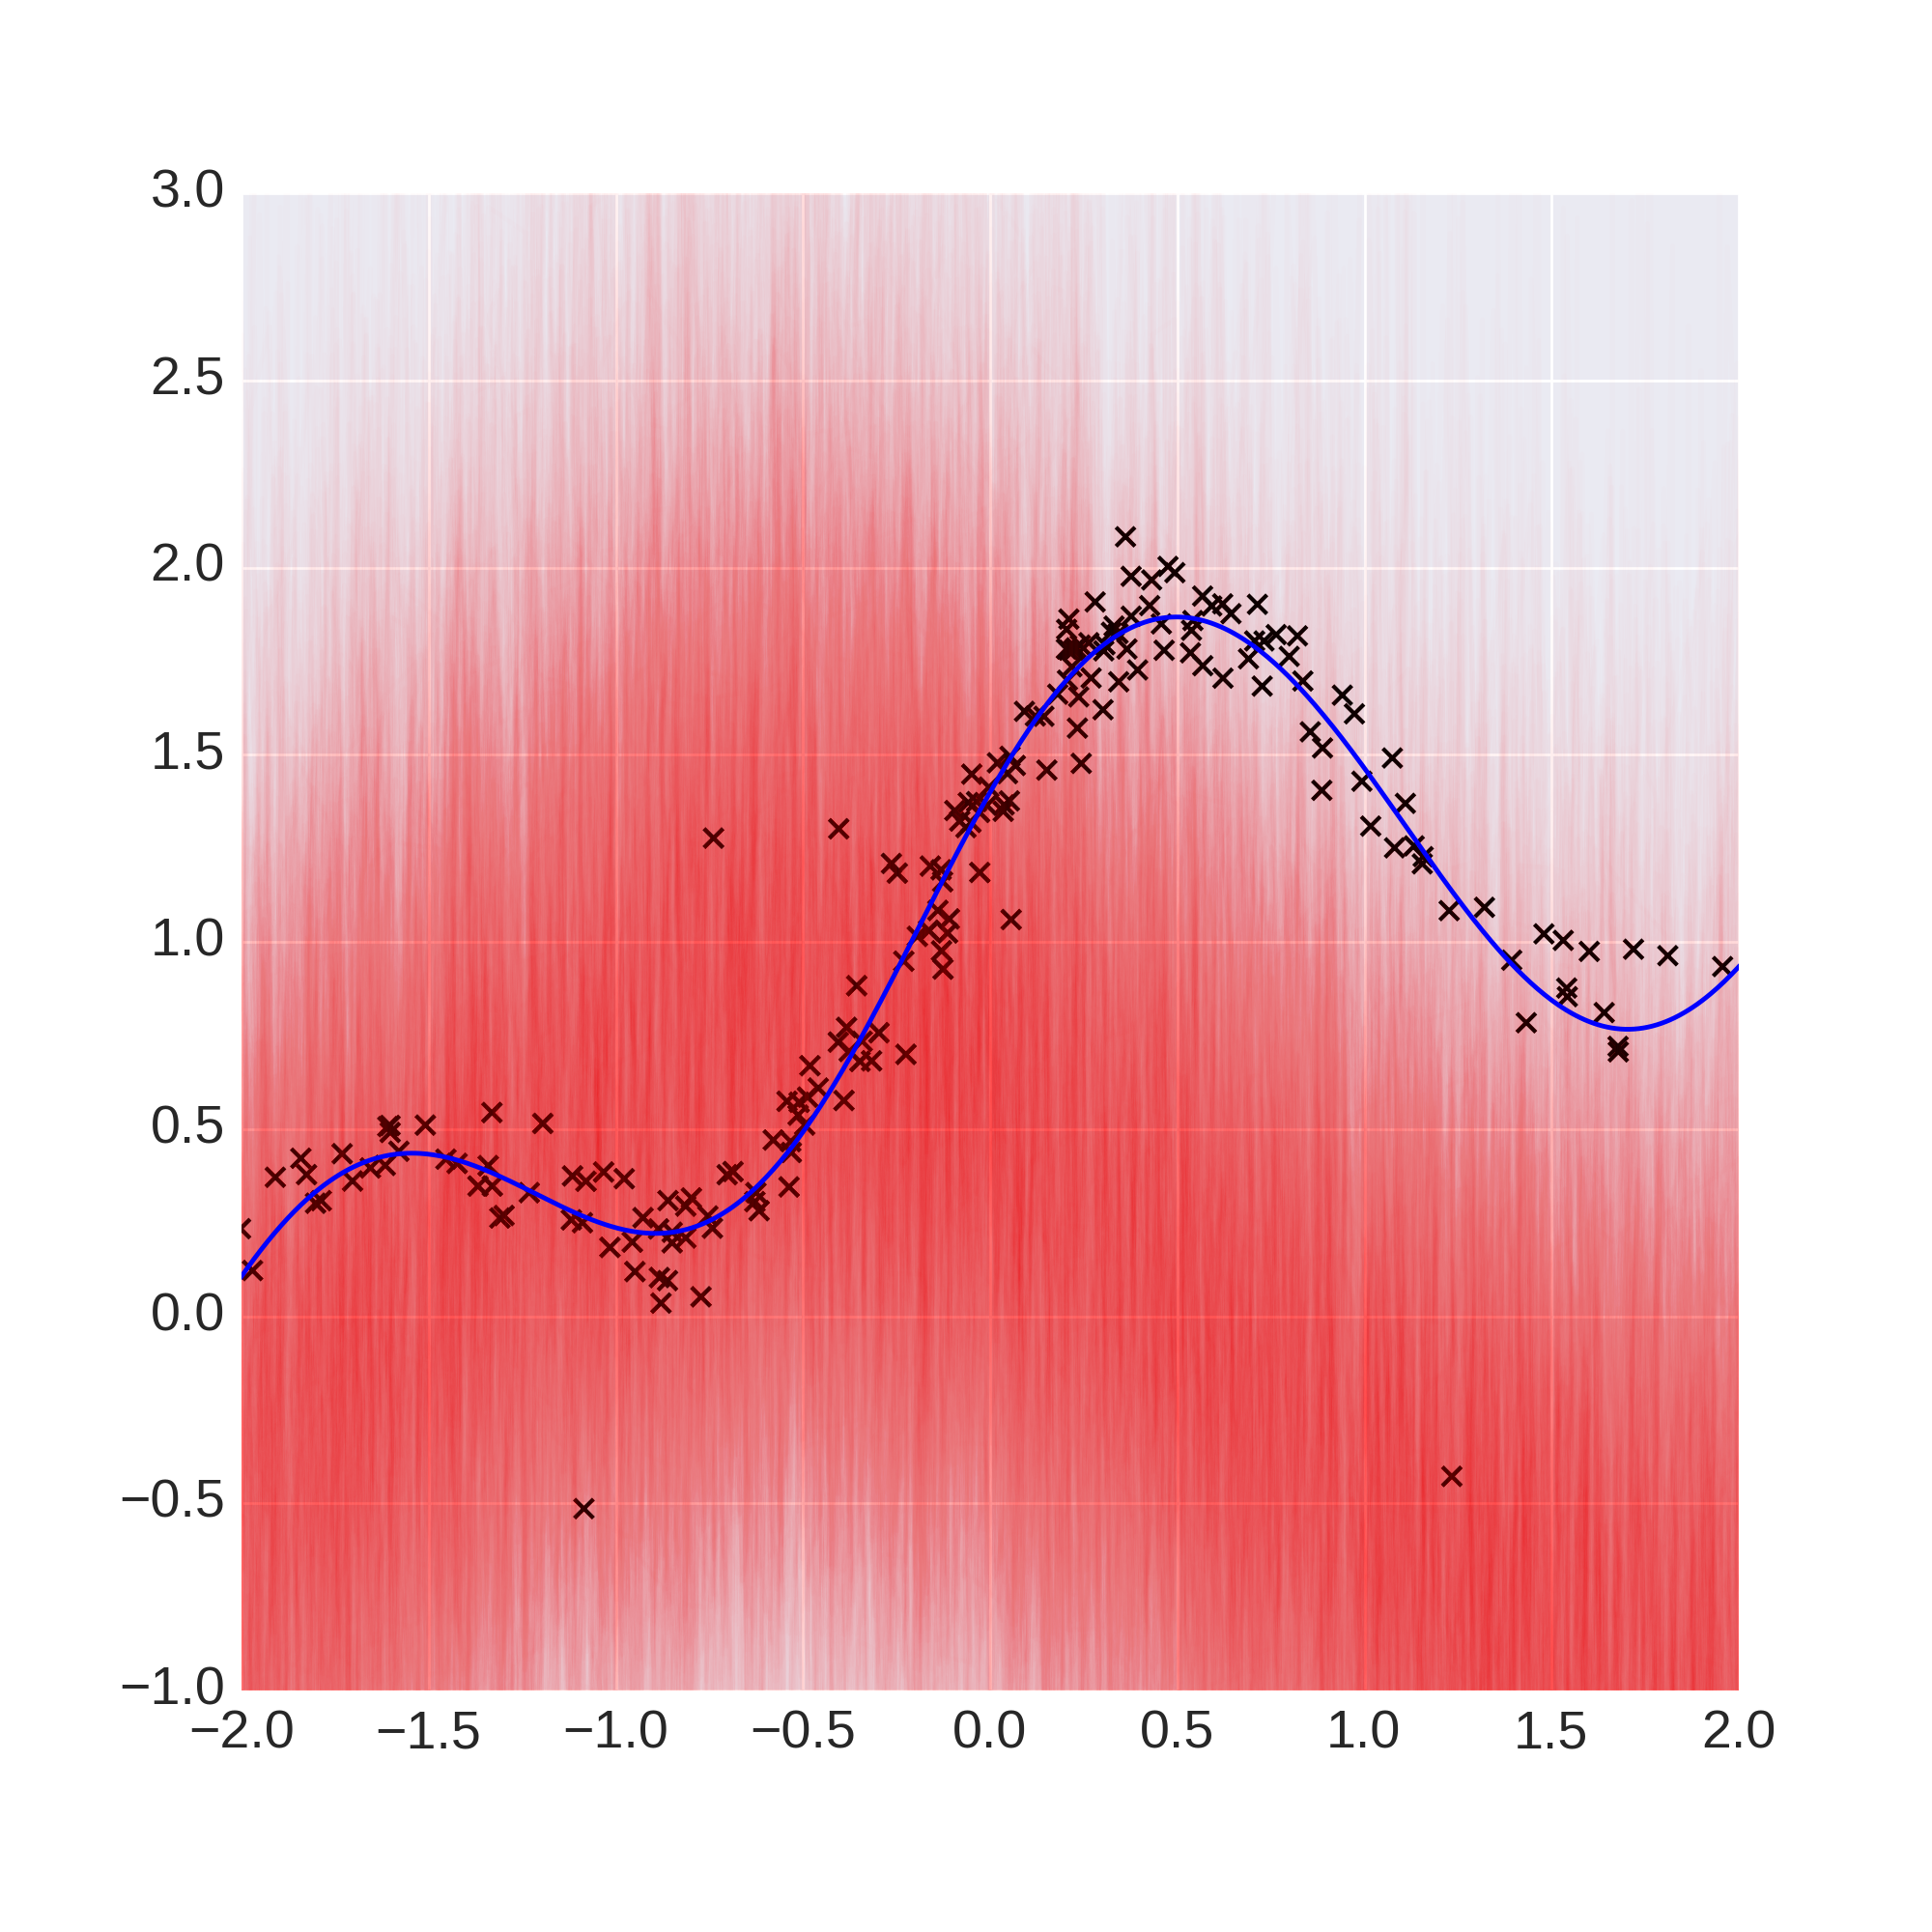
\includegraphics[height=7.5cm]{neal_se_2final.png}
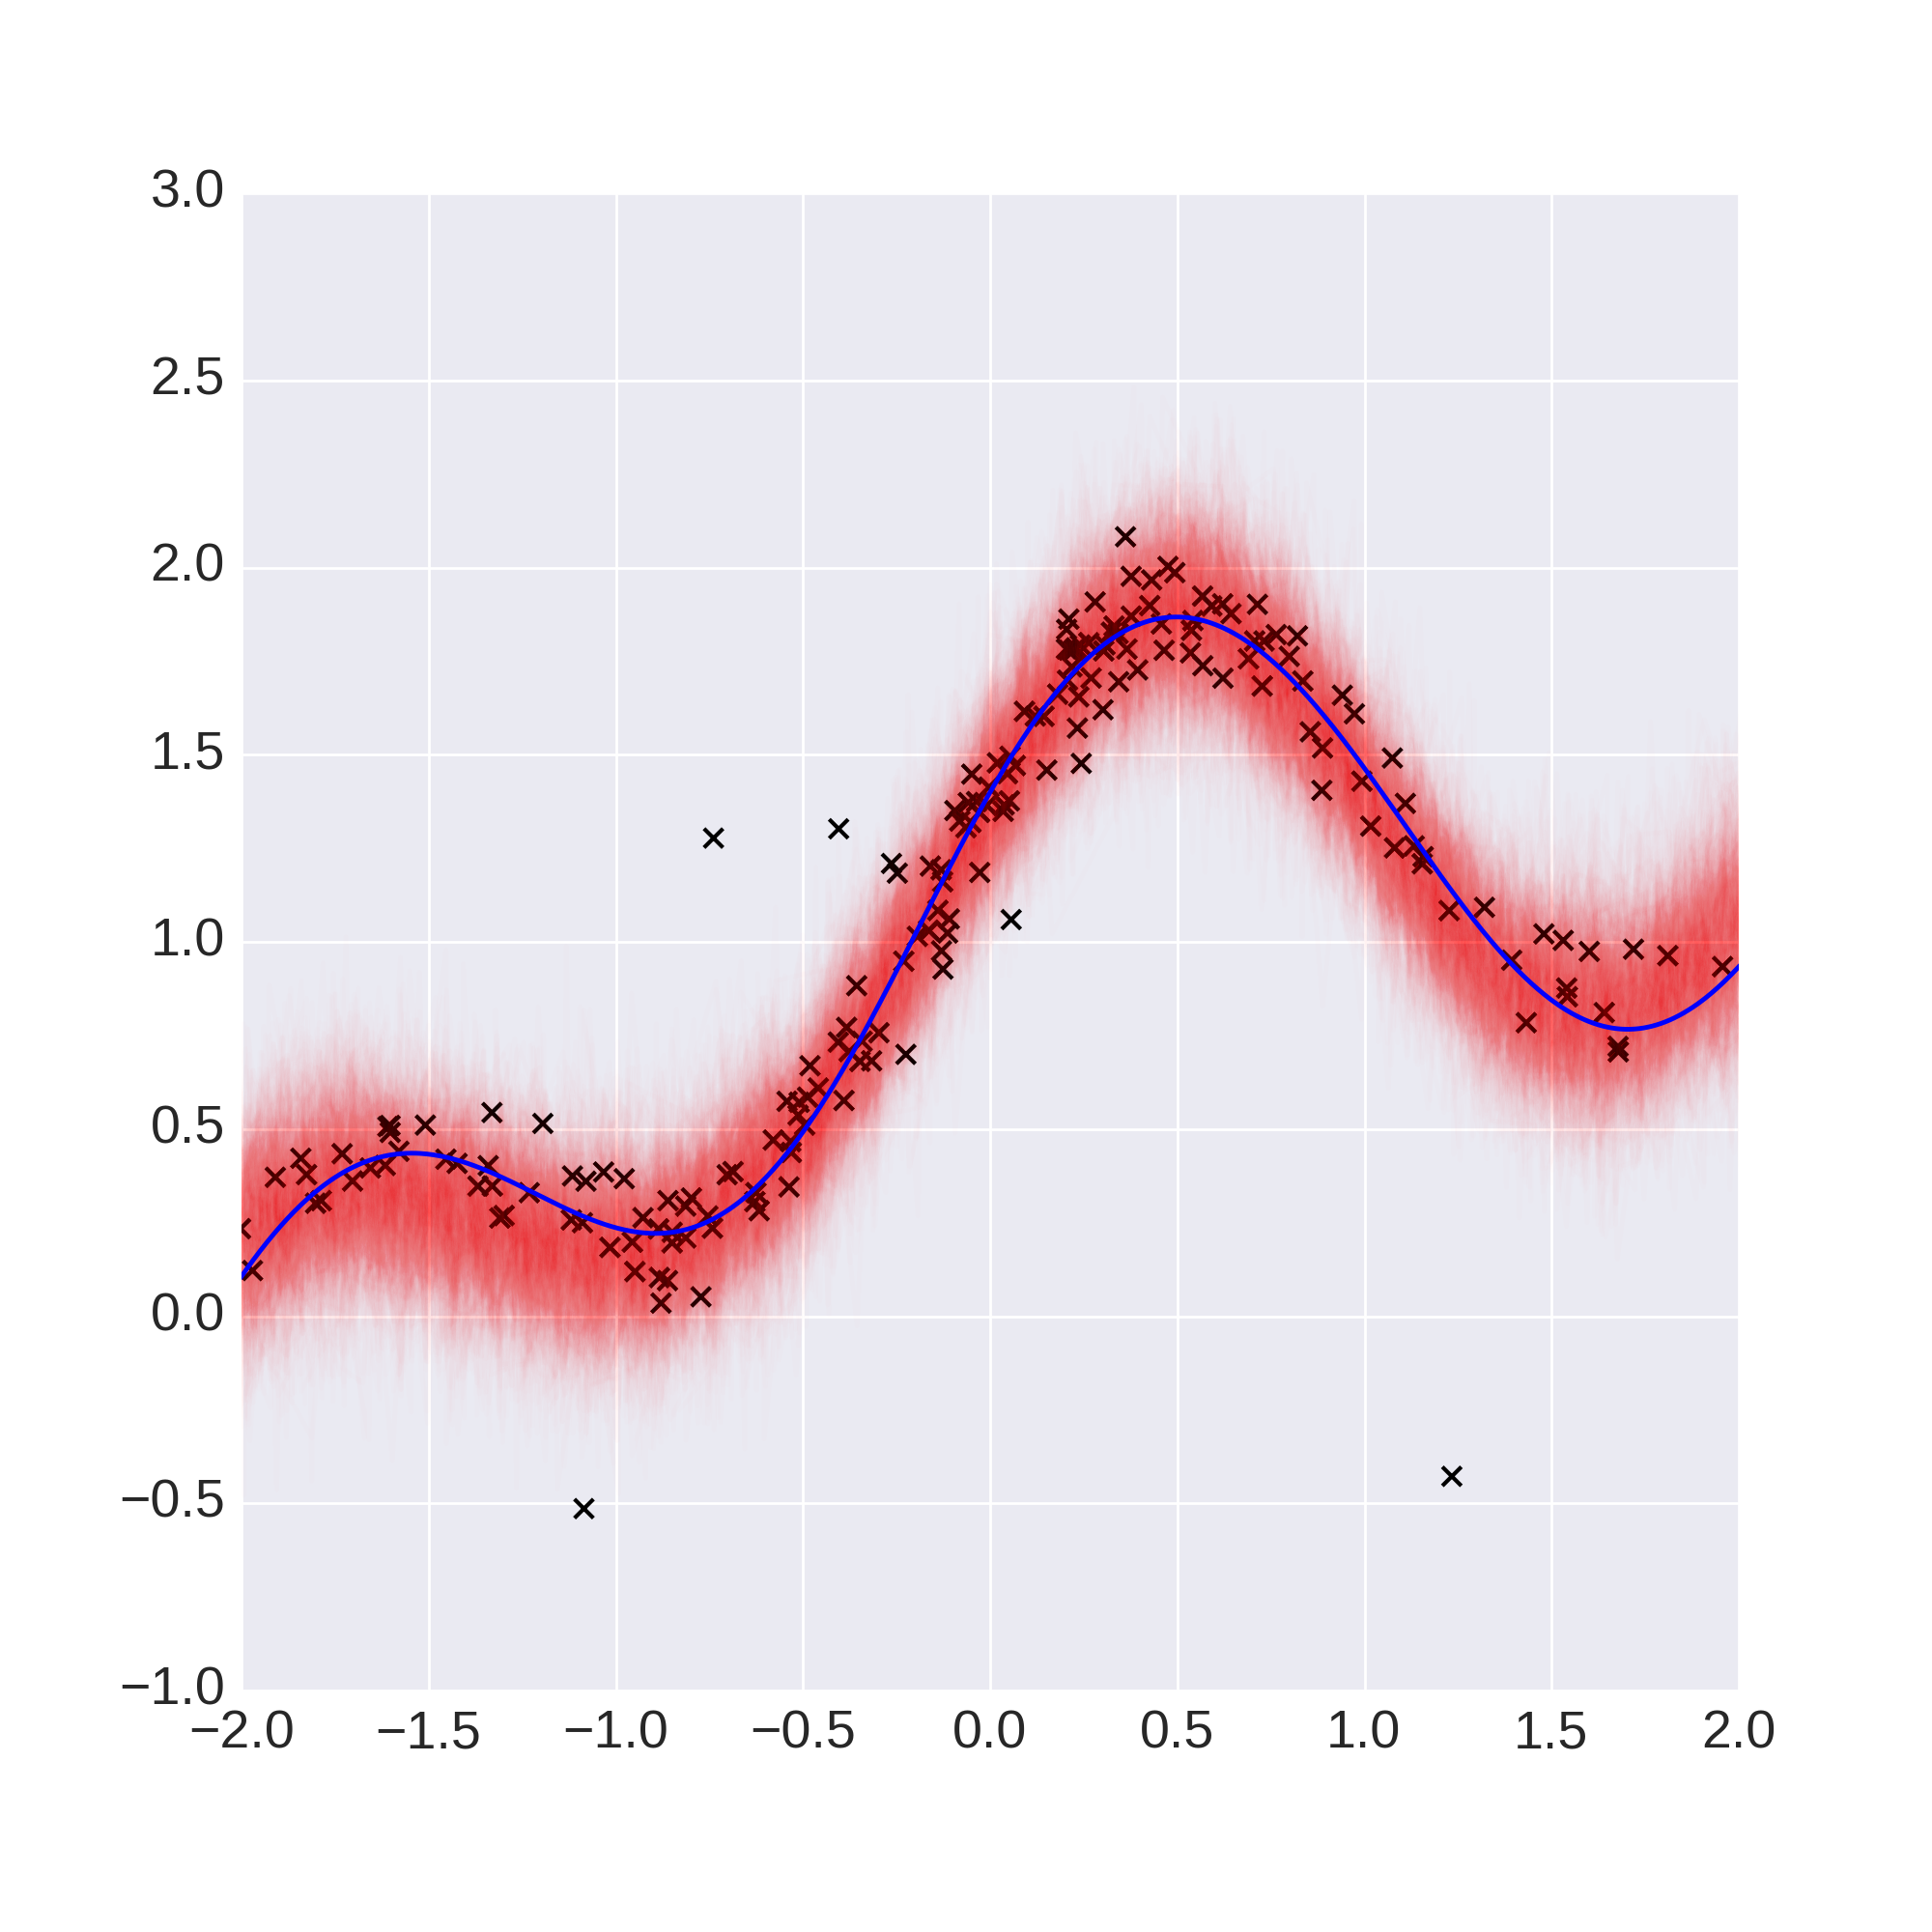
\includegraphics[height=7.5cm]{neal_se_3final.png}
\captionof{figure}{\color{DarkSlateGray} (a) depicts the hierarchical structure of the hyper-parameter as constructed in the work by Neal as a Bayesian Network. (b)-(d) shows \gpmem\ on Neal's example. We see that prior renders functions all over the place (a). After \gpmem\ observes a some data-points an arbitrary smooth trend with a high level of noise is sampled. After running inference on the hierarchical system of hyper-parameters we see that the posterior reflects the actual curve well. Outliers are treated as such and do not confound the GP.}\label{fig:neal}
\end{center}\vspace{1cm}


-------------------------------------------------


%----------------------------------------------------------------------------------------
%	Learning of Symbolic Structure
%----------------------------------------------------------------------------------------
\section*{Learning of Symbolic Structure}
\begin{center}\vspace{1cm}
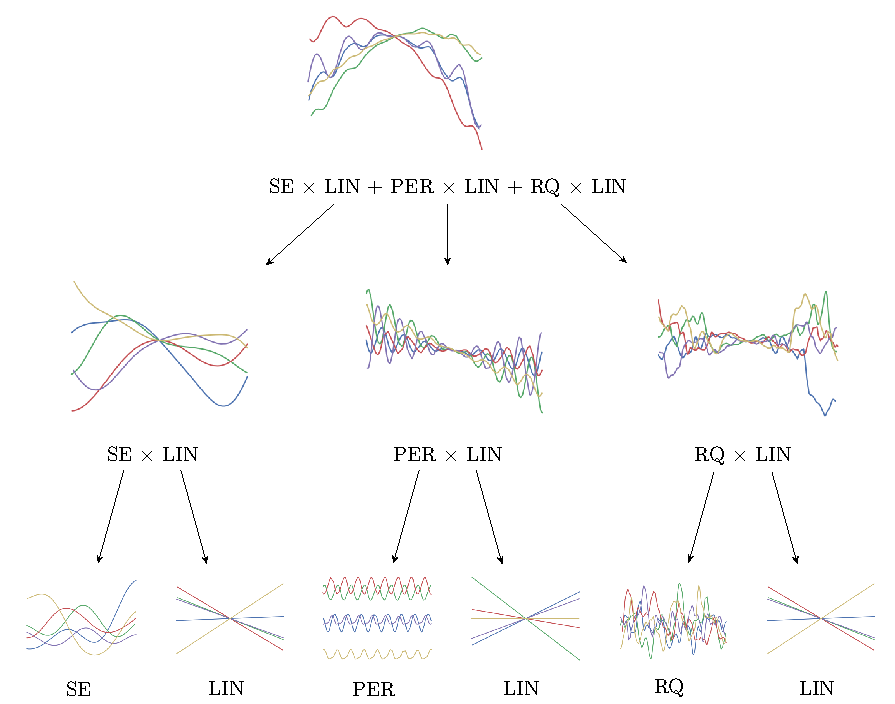
\includegraphics[width=0.8\linewidth]{parseTree.pdf}
\captionof{figure}{\color{DarkSlateGray} Composition of covariance function parsed using the example SE $\times$ LIN $+$ PER $\times$ LIN $+$  RQ $\times$ LIN}
\end{center}\vspace{1cm}

---------------------------------------------------------------------

%----------------------------------------------------------------------------------------
%	Bayesian Optimization
%----------------------------------------------------------------------------------------
\section*{Bayesian Optimization}

%\subsection*{Results}

\begin{center}\vspace{1cm}
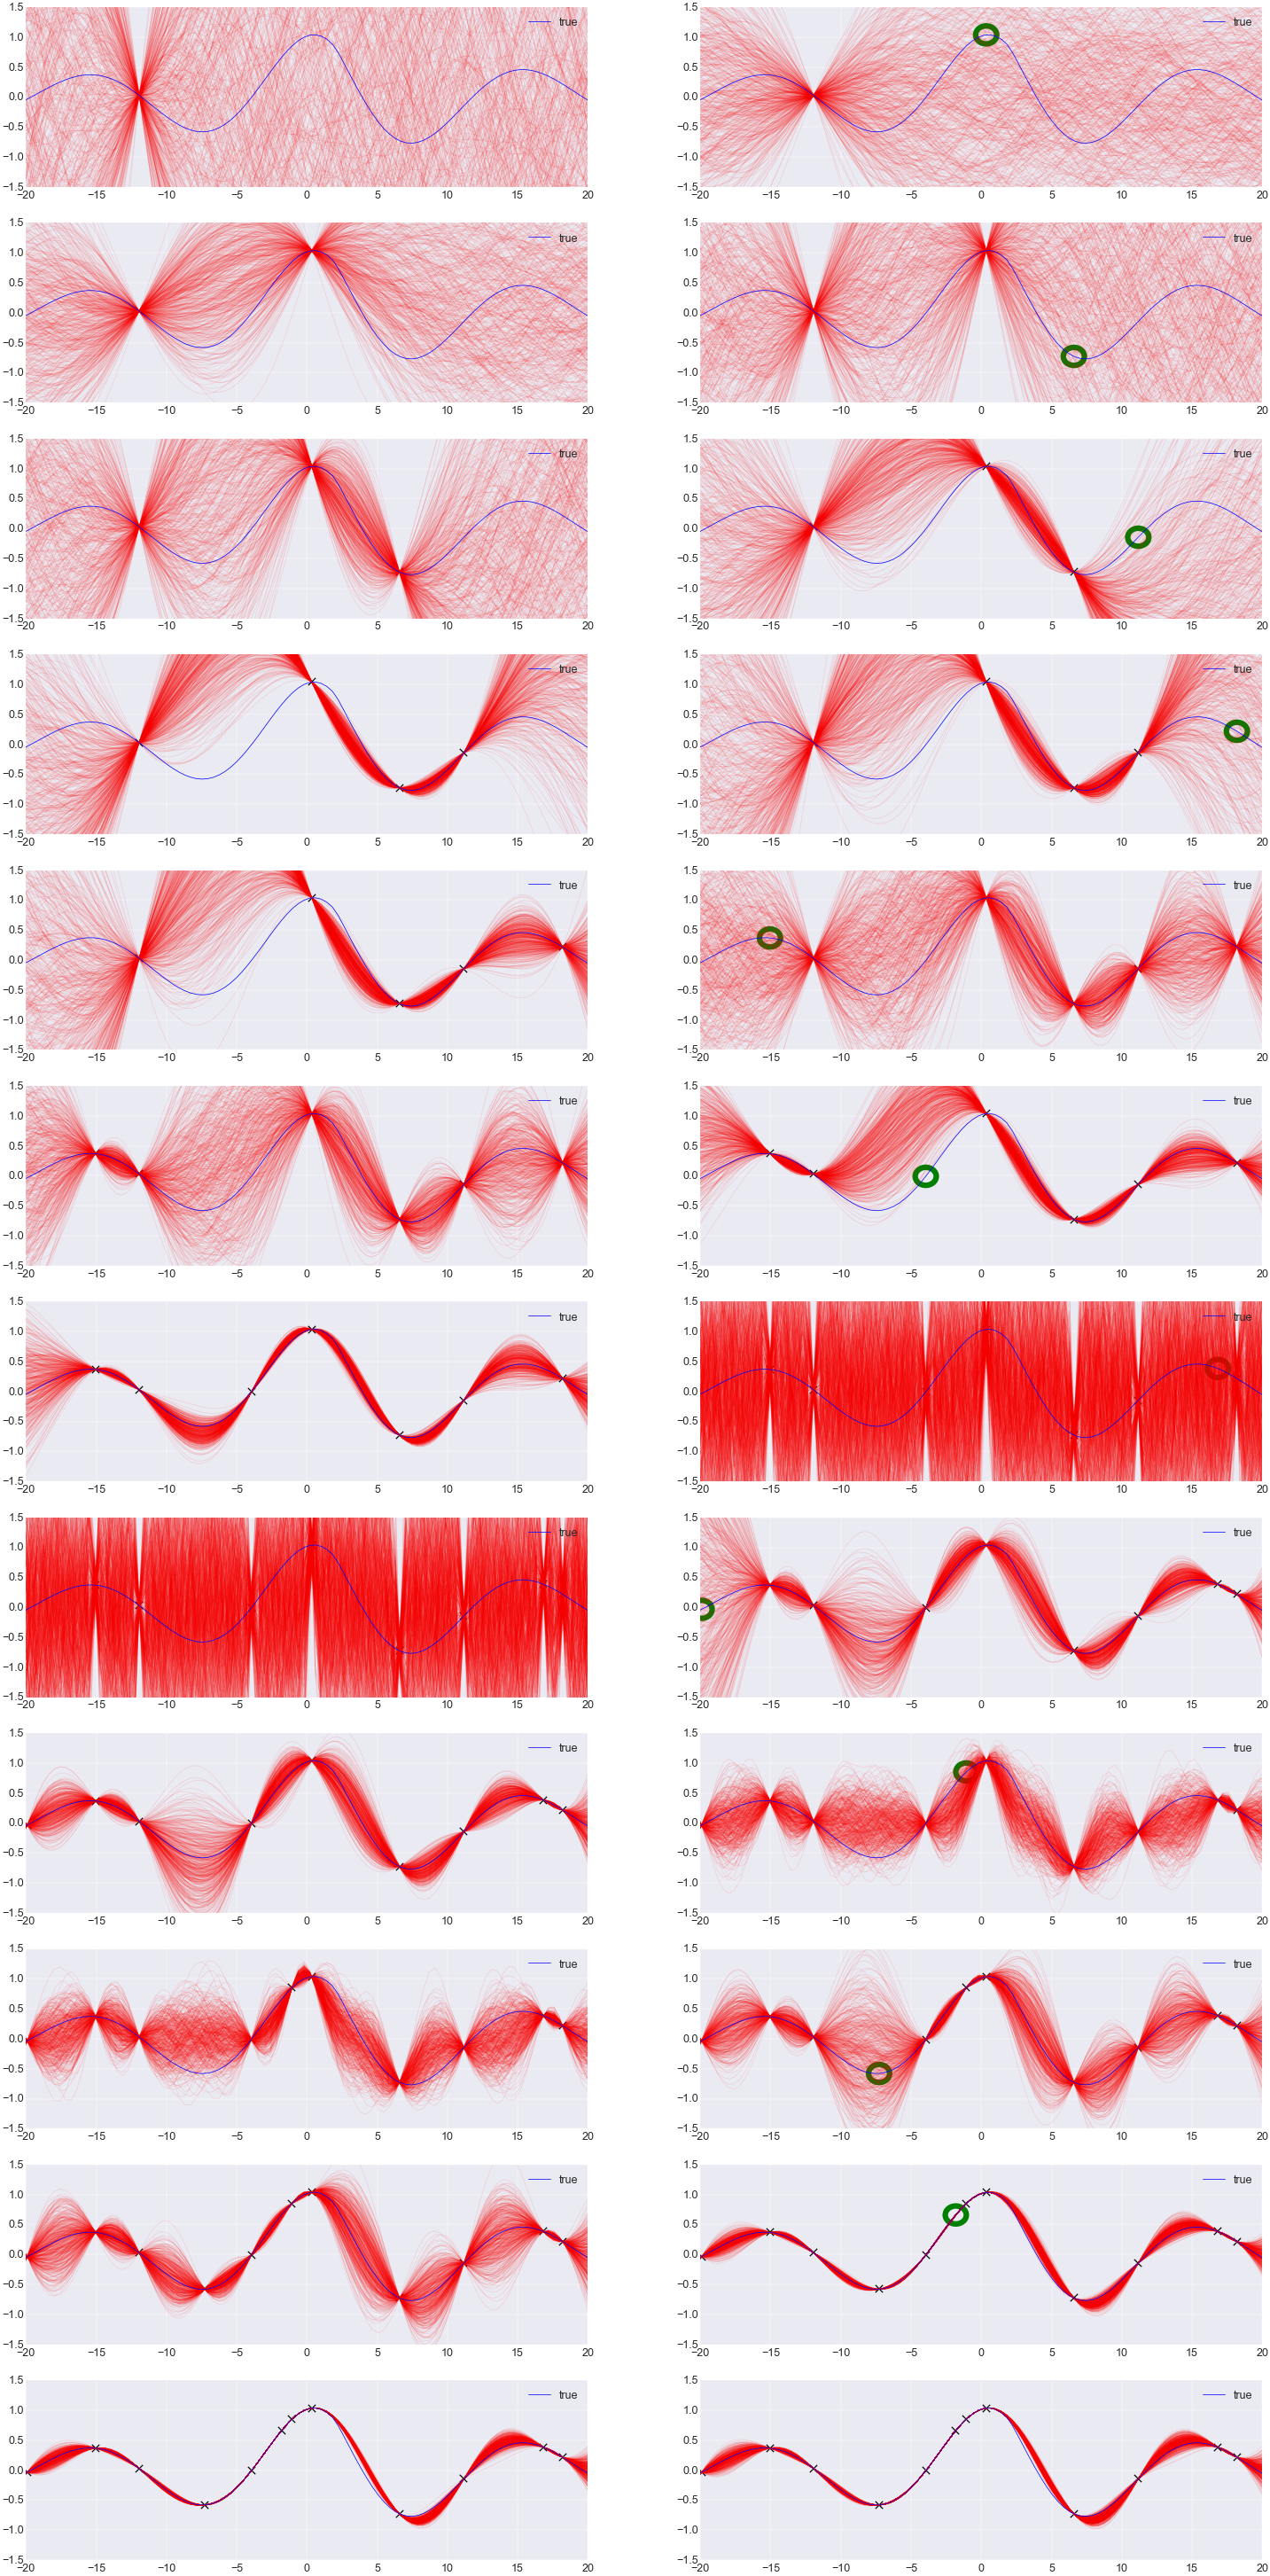
\includegraphics[width=0.6\linewidth]{BayesOpt_gpmem_sequence.png}
\captionof{figure}{\color{DarkSlateGray} Dynamics of Thompson sampling in Venture.
      The blue curve is the true function $V$, and the red region is a blending of 100 samples of the curve generated (jointly) by a GP-based emulator $V_\emu$.
      The left and right columns show the state of $V_\emu$ before and after hyperparameter inference is run on the new data, respectively.
      (We can see, for example, that after the seventh probe point, the Metropolis--Hastings sampler chose a ``crazy'' set of hyperparameters, which was corrected at the next inference step.)
      In the right column, the next chosen probe point is circled in green.
      Each successive probe point $a$ is the (stochastic) maximum of $V_\emu$, sampled pointwise and conditioned on the values of the previously probed points.
      Note that probes tend to happen at points either where the value of $V_\emu$ is high, or where $V_\emu$ has high uncertainty.} \label{fig:bayesopt-sequence}
\end{center}

   



\section*{Conclusions}

\begin{itemize}
\item Pellentesque eget orci eros. Fusce ultricies, tellus et pellentesque fringilla, ante massa luctus libero, quis tristique purus urna nec nibh. Phasellus fermentum rutrum elementum. Nam quis justo lectus.
\item Vestibulum sem ante, hendrerit a gravida ac, blandit quis magna.
\item Donec sem metus, facilisis at condimentum eget, vehicula ut massa. Morbi consequat, diam sed convallis tincidunt, arcu nunc.
\item Nunc at convallis urna. isus ante. Pellentesque condimentum dui. Etiam sagittis purus non tellus tempor volutpat. Donec et dui non massa tristique adipiscing.
\end{itemize}

\color{DarkSlateGray} % Set the color back to DarkSlateGray for the rest of the content

%----------------------------------------------------------------------------------------
%	FORTHCOMING RESEARCH
%----------------------------------------------------------------------------------------

%\section*{Forthcoming Research}

%Vivamus molestie, risus tempor vehicula mattis, libero arcu volutpat purus, sed blandit sem nibh eget turpis. Maecenas rutrum dui %blandit lorem vulputate gravida. Praesent venenatis mi vel lorem tempor at varius diam sagittis. Nam eu leo id turpis interdum %luctus a sed augue. Nam tellus.

 %----------------------------------------------------------------------------------------
%	REFERENCES
%----------------------------------------------------------------------------------------


\bibliographystyle{June2015} % Plain referencing style
\bibliography{sample} % Use the example bibliography file sample.bib

%----------------------------------------------------------------------------------------
%	ACKNOWLEDGEMENTS
%----------------------------------------------------------------------------------------

\section*{Acknowledgements}


%----------------------------------------------------------------------------------------

\end{multicols}
\end{document}